%----------------------------------------------------------------------------------------
%	PACKAGES AND THEMES
%----------------------------------------------------------------------------------------
\documentclass[aspectratio=169,xcolor=dvipsnames]{beamer}
\usepackage[english,russian]{babel}
\usetheme{Simple}

\usepackage{hyperref}
\usepackage{graphicx} % Allows including images
\usepackage{booktabs} % Allows the use of \toprule, \midrule and \bottomrule in tables

%----------------------------------------------------------------------------------------
%	TITLE PAGE
%----------------------------------------------------------------------------------------

% The title
\title{Анализ эффективности нейросетевых вычислений с учетом аппаратных возможностей платформ}
\subtitle{Курсовая работа}

\author[Pin-Yen] {Бинцаровский Леонид Петрович}
\institute[NTU] % Your institution may be shorthand to save space
{
    % Your institution for the title page
    Белорусский государственный университет\\
    ФПМИ, ДМА, 3 курс\\
    руководитель: старший преподаватель Пирштук Д. И.
    \vskip 3pt
}
\date{Минск, 2024} % Date, can be changed to a custom date


%----------------------------------------------------------------------------------------
%	PRESENTATION SLIDES
%----------------------------------------------------------------------------------------

\begin{document}

\begin{frame}
    % Print the title page as the first slide
    \titlepage
\end{frame}

% \begin{frame}{Overview}
%     % Throughout your presentation, if you choose to use \section{} and \subsection{} commands, these will automatically be printed on this slide as an overview of your presentation
%     \tableofcontents
% \end{frame}

%------------------------------------------------
\section{First Section}
%------------------------------------------------

\begin{frame}{Сферы применения нейронных вычислений}
    \begin{columns}[c] % The "c" option specifies centered vertical alignment while the "t" option is used for top vertical alignment

        \column{.45\textwidth} % Left column and width
        \begin{itemize}
            \item Компьютерное зрение
            \item Обработка естественного языка
            \item Медицинская диагностика
            \item Финансовый анализ
            \item Управление беспилотниками
        \end{itemize}

        \column{.5\textwidth} % Right column and width
        \begin{figure}[h]
            \center{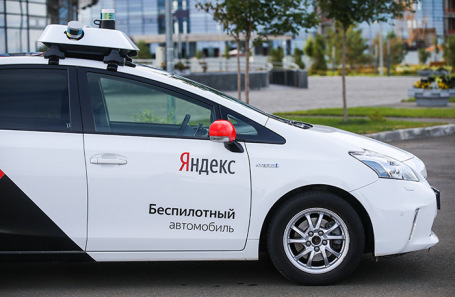
\includegraphics[width=\linewidth]{images/yandeks.jpg}}
            \label{ris:ORTModelData}
        \end{figure}
        
    \end{columns}
\end{frame}

%------------------------------------------------

\begin{frame}{Анализ эффективности инференса провайдеров будет проводиться на моделях}
    \begin{enumerate} 
      \item Mediapipe;
      \item Selfie\_segmentation;
      \item SINet\_softmax\_simple;
      \item pphumanseg\_fp32;
      \item rvm\_mobilenetv3\_fp32.
    \end{enumerate}
\end{frame}

%------------------------------------------------

\begin{frame}{Постановка задачи}
    Для анализа эффетикности нейросетевых вычислений выбранных моделей, будут использоваться:

    \begin{block}{Фреймворк}
        ONNX Runtime
    \end{block}

    \begin{block}{Провайдеры}
        DefaultCPU, DirectML, QNN, OpenVINO и oneDNN. 
    \end{block}

    \begin{block}{Язык программирования, среда разработки и операционная система}
        С++, Visual Studio и Windows
    \end{block}
\end{frame}


%------------------------------------------------

\begin{frame}{Основные элементы тестового инференса}
    \begin{columns}[c] % The "c" option specifies centered vertical alignment while the "t" option is used for top vertical alignment

        \column{.45\textwidth} % Left column and width
        \begin{figure}[h]
            \center{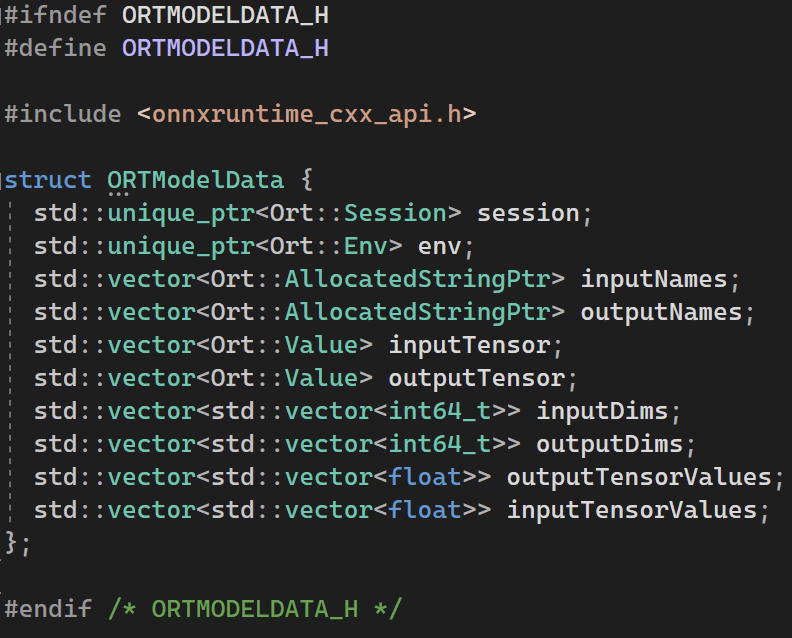
\includegraphics[width=0.9\linewidth]{images/ORTModelData.png}}
            \label{ris:ORTModelData}
        \end{figure}

        \column{.5\textwidth} % Right column and width
        \begin{enumerate}
            \item Структура ORTModelData
            \item Структура FilterData
            \item Базовые классы модели Model и ModelBCHW
            \item Классы каждой модели 
            \item Функции createOrtSession и runFilterModelInferece
            \item Класс BackgroundFilter
        \end{enumerate}

    \end{columns}
\end{frame}

%------------------------------------------------

\begin{frame}{Описание методики тестирования}
    \begin{columns}[c] % The "c" option specifies centered vertical alignment while the "t" option is used for top vertical alignment

        \column{.45\textwidth} % Left column and width
        \begin{figure}[h]
            \center{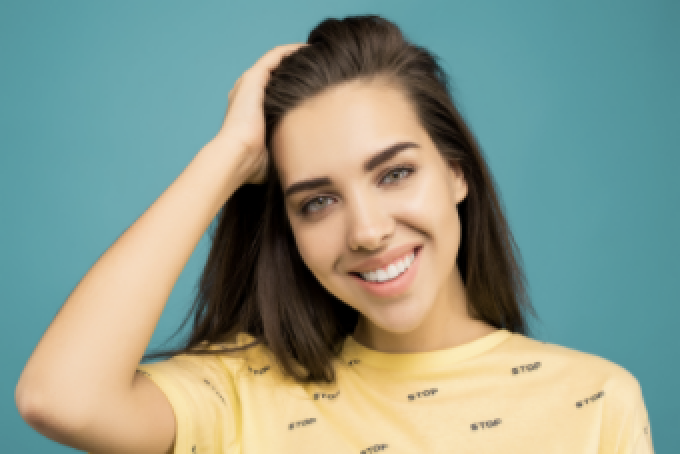
\includegraphics[width=0.9\linewidth]{images/input.png}}
            \label{ris:ORTModelData}
        \end{figure}

        \column{.5\textwidth} % Right column and width
        \begin{enumerate}
            \item Macbook на чипе M1
            \item Виртуальная машина windows 11
            \item Фиксированное входное изображение
            \item 1 и 3 ядра CPU
            \item Измерялось минимальная, максимальная и средняя скорость инференса
            \item "Разогев" 100 и 300 итераций
            \item 3000 основных итераций 
        \end{enumerate}

    \end{columns}
\end{frame}

%------------------------------------------------
\section{Second Section}
%------------------------------------------------

\begin{frame}{Анализ результатов для модели Mediapipe}
    \begin{columns}[c] % The "c" option specifies centered vertical alignment while the "t" option is used for top vertical alignment

        \column{.45\textwidth} % Left column and width
        \begin{figure}[h]
            \center{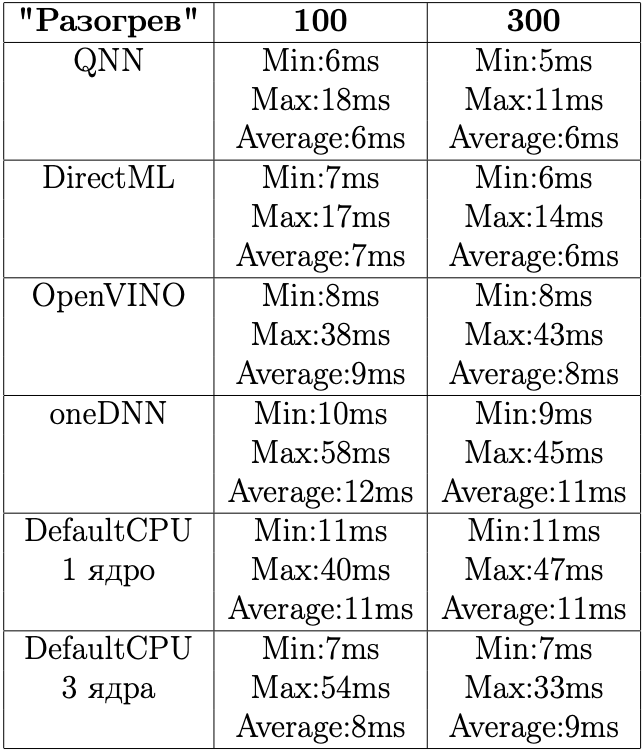
\includegraphics[width=0.8\linewidth]{images/mediapipe.png}}
            \label{ris:mediapipe}
        \end{figure}

        \column{.5\textwidth} % Right column and width
        В данной таблице представлены результаты инференса модели mediapipe. Лучшая скорость была получена при использовании провайдера QNN с количеством итераций цикла "Разогрева" равными 300.

    \end{columns}
\end{frame}

%------------------------------------------------

\begin{frame}{Анализ результатов для модели pphumanseg\_fp32}
    \begin{columns}[c] % The "c" option specifies centered vertical alignment while the "t" option is used for top vertical alignment

        \column{.45\textwidth} % Left column and width
        \begin{figure}[h]
            \center{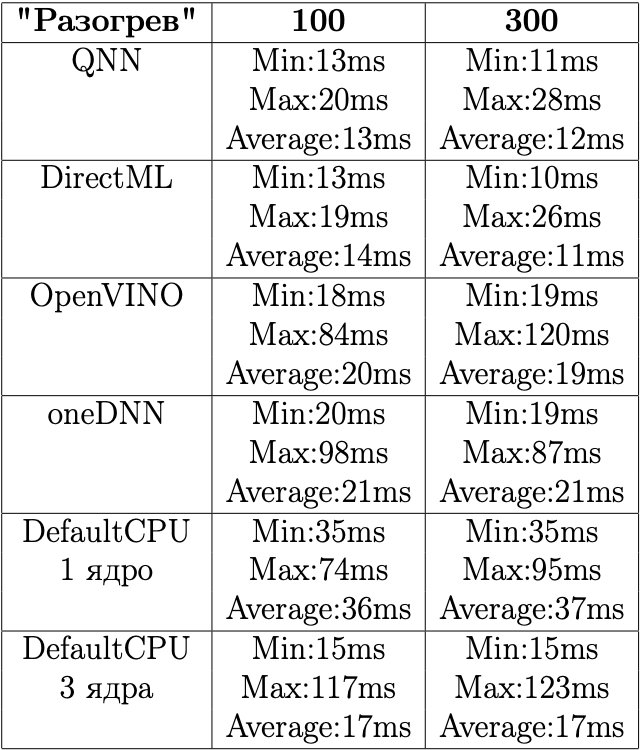
\includegraphics[width=0.8\linewidth]{images/pphumanseg.png}}
            \label{ris:pphumanseg}
        \end{figure}

        \column{.5\textwidth} % Right column and width
        В данной таблице представлены результаты инференса модели pphumanseg\_fp32. Лучшая скорость была получена при использовании провайдера DirectML с количеством итераций цикла "Разогрева" равными 300.

    \end{columns}
\end{frame}

%------------------------------------------------

\begin{frame}{Выводы}
    \begin{itemize}
        \item Сделан краткий обзор фреймворка ONNX Runtime и провайдеров OpenVINO, DirectML, oneDNN, QNN и DefaultCPU;
        \item Реализованы классы для кросс-платформенного инференса моделей mediapipe, Selfie\_segmentation, pphumanseg\_fp32, SINet\_softmax\_simple и rvm\_mobilenetv3\_fp32;
        \item Реализованы платформозависимые компоненты: DirectML, OpenVINO, oneDNN, QNN;
        \item Создана тестовая программа для замера скорости инференса выбранной модели;
        \item Проведено сравнение скорости инференса моделей в зависимости от используемого провайдера или количеста ядер CPU.
    \end{itemize}
\end{frame}

%----------------------------------------------------------------------------------------

\end{document}